\chapter{Improvements to the Basic Project}

In the previous chapter, the focus was on creating a project that can target a dual-core STM32 microcontroller. It was however only a basic "Hello World" type project that can be massively improved upon. In this chapter, I will demonstrate the steps that were taken before attempting to build a proper example project.

\section{UART}

Establishing a serial connection between the target MCU and the host PC is usually the most important first step at the start of a new embedded project. While a UART line may not have full debugging capabilities, it allows for quick and relatively easy text-based communication with the host. These traces are a very effective tool in determining where a program gets stuck in a loop or panics.

The following code brings up the UART interface that is linked to the ST-Link connector on the board. In this project, this UART interface is used for debugging purposes, so only the rx line is not in use. Rust generates warnings for variables that are not used, this can be avoided by prepending an underscore to the unused variable. The serial line is configured to operate with 19200 baudrate and without flow control.

\begin{lstlisting}[language=Rust,frame=single,float=!ht,style=customrust,label={lst:uart-bringup},caption={UART Interface Configuration}]
    let tx = gpiod.pd8.into_alternate();
    let _rx = gpiod.pd9.into_alternate();
    let serial = dp
        .USART3
        .serial((tx, _rx), 19200.bps(), ccdr.peripheral.USART3, &ccdr.clocks)
        .unwrap();
    let (mut tx, _rx) = serial.split();
\end{lstlisting}

\section{Debugger}

Using traces on a serial line for detecting errors in the code may not be sufficient in all cases. Moreover, the overhead of printing to this peripheral can disrupt the timing of certain parts of the program. In these cases configuring a debugger becomes a necessity.

All STM32 development boards are equipped with an on-board ST-Link debugger. ST-Link connects to the host PC through a USB interface. The ST-Link can facilitate debugging through different modes of communication for example single-wire interface module (SWIM), serial wire debugging (SWD), and Joint Test Action Group (JTAG) of which the latter is used most often.

The official IDE provided by STM, STMCubeIDE includes full debugging capabilities, however, these tools can only handle C and C++ code. The Rust ecosystem does not currently have a standard tool nor does STM provide debugging tools for other languages. Most often though Rust developers will use openocd, gdb, and VSCode.

\subsection{OpenOCD}

Open On-Chip Debugger (OpenOCD) is an open-source tool that provides debugging and in-system programming capabilities for embedded devices such as this STM32 microcontroller. It serves as a bridge between the development environment on a host machine and the microcontroller's hardware, facilitating the debugging process.

OpenOCD supports various hardware interfaces, such as JTAG, SWD, and various proprietary interfaces provided by different microcontroller vendors. These interfaces are crucial for establishing a connection between the host machine and the microcontroller, enabling the exchange of debugging information. The software can be configured to the parameters of the target device, such as the CPU architecture, target voltage, and other specific settings. This ensures that the debugger communicates effectively with the microcontroller.

OpenOCD acts as a GDB (GNU Debugger) server, providing a standardized interface for debugging tools. GDB is a full-fledged debugger but only its server part is used in this configuration. OpenOCD enables GDB to connect to the target microcontroller, allowing developers to interact with and debug their code. The program also supports in-system programming, allowing users to flash the firmware onto the memory of the microcontroller. This is essential for updating or loading new firmware onto the device during the development and debugging process, however, it is also possible to start debugging without flashing in new software, which is ideal for our case as the flashing process for this project is non-trivial due to the two cores.

OpenOCD can be integrated with various Integrated Development Environments and toolchains, providing a seamless debugging experience for developers using different development environments. Being an open-source project, it benefits from a vibrant community that contributes to its development and supports a wide range of hardware platforms. It also allows users to customize and extend its functionality based on their specific debugging requirements.

In the case of this project, the OpenOCD configuration is already provided for the evaluation board \cite{OpenocdConfigFile}.

\subsection{GDB}

The GNU Debugger (GDB) is an open-source debugger most often used in Linux and embedded development. GDB has a command line interface and can only be used from a terminal so in recent times it is usually replaced by a more modern debugger with a graphical user interface. These debuggers are provided by the chip manufacturer most of the time. However, as Rust support for STM32 microcontrollers is community driven, selecting GDB as a debugger is a logical step.

GDB communicates with OpenOCD, which acts as a hardware interface and facilitates communication between the host machine and the Cortex-M microcontroller. OpenOCD establishes the link between GDB and the target device, allowing GDB to exert control over the microcontroller for debugging purposes. The debugger supports ARM architectures, including Cortex-M. It understands the specific characteristics and features of these architectures, allowing developers to debug Rust applications targeting Cortex-M microcontrollers effectively.

GDB has all the features of a modern debugger, only developers need to be familiar with the proper commands. It supports symbolic debugging, enabling developers to use high-level constructs like variable names and function names during the debugging process. This abstraction makes it easier to understand and troubleshoot code behavior at a higher level of abstraction. GDB allows developers to set breakpoints at specific lines or functions in the code. It also supports step-by-step execution, enabling users to navigate through the code, line by line, to identify and diagnose issues. During debugging sessions, GDB provides the capability to inspect and modify variable values in real time. This feature is crucial for understanding the state of the program and making runtime adjustments as needed. GDB allows developers to evaluate expressions and execute commands during a debugging session. This functionality is valuable for dynamically assessing variables or executing specific code snippets to gain insights into the program's behavior. And most importantly as Rust is an LLVM (Low-Level Virtual Machine) compatible language it can fully utilize all of the features of an LLDB (Low-Level Debugger) such as the GNU Debugger.

\subsection{VSCode}

The final component of this debugger toolchain setup is Visual Studio Code. While VSCode in and of itself is just a feature-rich text editor, with the proper extensions and settings, it can act as a full-fledged IDE including building, flashing, and remote debugging projects. In the previous section, GDB was introduced as a complete debugger but it is still missing a convenient graphical user interface. VSCode can provide this interface and handle the GDB commands that need to be executed for the provided utilities.

To configure VSCode correctly, the project must contain at least two additional files placed in the root of the project into a \mycode{.vscode} folder and the Cortex-Debug extension \cite{CortexDebug}. The first file is \mycode{tasks.json}. This file can contain multiple tasks that can be executed by commands in Visual Studio Code. In a project like this, normally two tasks are needed. One is to build the project using \mycode{cargo} commands and another one that converts the resulting ELF file into a format that can be loaded onto the microcontroller using an interface supported by OpenOCD. The other file \mycode{launch.json} contains the settings and commands that will start and handle the debugging session. This configuration file holds the path to the executable that will be used for the debugging session, the OpenOCD config file, and some pre- and postlaunch commands. Using these two files, the debug button in VSCode will build an image with the current source files, load it onto the memory of the microcontroller, and start the debugging session. The developer is then able to place breakpoints, stop and start the code as well, and step through it line by line.

\section{Cargo Makefile}

In the previous iteration of this project, a Makefile was added around the Cargo project to generate binary and HEX images from the original ELF output. However, as this project is already using the Rust ecosystem it may be beneficial to replace the traditional Makefile with a cargo equivalent and reduce the number of external dependencies of this project. The normal cargo build flow can be supplemented with a \mycode{build.rs} file at the root of the crate. This file will compile and run before the source files are compiled when using the \mycode{cargo build} command. However, in our case, the build process contains operations after the build is finished, so another solution is necessary.

The \mycode{cargo-make} \cite{CargoMake} project aims to replace the GNU Makefile with a "rusty" alternative. The tool can be installed using cargo with the command \mycode{cargo install cargo make} and then it can be invoked similarly to GNU make \mycode{cargo make <task>}, where a task is similar to a target in a traditional Makefile. Tasks can be described in a file placed at the crate root titled \mycode{Makefile.toml}. Similarly to how the project can be configured, the build related tasks are to be described in a TOML format. Variables can be set in the \mycode{[env]} section, and tasks can be defined in their own sections under the \mycode{tasks} section. Below is a minimal \mycode{Makefile.toml} file which builds a simple Rust project with the \mycode{cargo make} command.

\begin{lstlisting}[language=C,frame=single,float=!ht,label={lst:cargo-task-example},caption={Cargo Make Task Example}]
    [env]
    OUTPUT_FILENAME = "example"

    [tasks.build]
    clear = true,
    command = "cargo"
    args = [
        "build",
        "--bin", "${OUTPUT_FILENAME}"
    ]

    [tasks.default]
    clear = true,
    dependencies = [ "build" ]
\end{lstlisting}

Some tasks have default defines, for example, the \mycode{build} task would just execute the command \mycode{cargo build}, and the \mycode{clear = true} line makes sure that all parts of these default definitions are overwritten. The dependencies field array lists all the tasks that need to be executed before the current one can run. These dependencies are evaluated in the listed order. For our purposes, cargo-make is a good replacement for a GNU Makefile, but in reality, it lacks one important feature that is present in normal make. Currently, all dependent tasks are executed before the current one, even if their output is more recent than its requirements. This is a great advantage of Makefiles and a necessity in every build system. The longest part of the build in this project is still the invocation of \mycode{cargo build} command, which only recompiles files with changes, so the solution is still acceptable in our case. However, cargo-make is still being developed continually so upgraded dependency handling may be possible in the near future.

\section{Flashing}

So far various ways of flashing our software onto the microcontroller have been discussed. \mycode{cargo-flash} seemed to be the most fitting for this project, but using tools provided by ST just seemed more convenient. Setting up a cargo makefile made me reevaluate this aspect of the project and take another look at command line utilities so the deployment process could be automated. The fix to the previously mentioned error in \mycode{st-flash} is still not released at the time of writing, \mycode{cargo-flash} seemed to be the only way forward. It is still only able to flash to one core at a time, however at this stage of the project, where we can be sure that soft resetting the microcontroller will guarantee a steady state, single-core flashing will be enough. So three more tasks were added to \mycode{Makefile.toml}, one for flashing each core, and a deploy task that combines these two and builds the whole project.

\begin{lstlisting}[language=C,frame=single,float=!ht,label={lst:cargo-make-deploy},caption={Cargo Tasks to Flash the MCU}]
    [tasks.deploy0]
    clear=true
    command = "cargo"
    args = [
        "flash",
        "--elf",
        "${ELF_FILE_0}",
        "--chip",
        "STM32H745ZITx"
    ]

    [tasks.deploy1]
    clear=true
    command = "cargo"
    args = [
        "flash",
        "--elf",
        "${ELF_FILE_1}",
        "--chip",
        "STM32H745ZITx"
    ]

    [tasks.deploy]
    clear = true
    dependencies = ["all", "deploy0", "deploy1"]
\end{lstlisting}

Using this configuration both cores of the microcontroller can be updated after building the current state of the project using a single command: \mycode{cargo make deploy}.

\section{Docker Image}

\subsection{Docker introduction}
The problem of dependency hell \cite{DependencyHell} usually means that libraries used in our code can be dependent on various versions of each other. However, the concept can be expanded to compiler tools and toolchains in an embedded project where, for example, the version of the compiler or debugger could be locked by the manufacturer of the microcontroller. This is especially a problem for developers who are working on multiple projects or hardware as development tools are sometimes installed system-wide. So what can be the solution when multiple projects collide and their dependencies cannot or hardly co-exist on the same system?

Docker is a platform that provides a means to create and run applications in containers. Containers are portable, lightweight, and self-sufficient units that encapsulate software and its dependencies. This allows us to use the same tools during development and deployment across multiple systems. In embedded software development all the tools used for compiling, flashing, and debugging our code can be included in the container with the libraries these programs depend on. Until Docker became widespread the only way to do this separation was to create virtual machines for each of our projects. Setting up and building docker containers is much faster than the installation of a virtual machine \cite{VMVsDocker}. Our project does not use significant resources and can sit comfortably on the host operating system with the Docker engine providing the isolation.

\subsection{Utilizing Docker in the project}

\subsubsection{Dockerfile}

Using Docker for this project is a two-step process. First, we need to create a Docker image that can build, flash, and debug our applications, then we need to configure our editor, VSCode in this case, to work with this container.

To use Docker with a project, we need to place a \mycode{Dockerfile} to the root of it. A \mycode{Dockerfile} is basically a list of instructions on how to build the image. It usually starts with a \mycode{FROM} statement, which signals to the docker engine that our container is derived from another one. In our case, it will be derived from the official Rust container. Also, the version of this container can be fixed here so the dependencies will not change as newer versions are released to the Docker container store.

\begin{lstlisting}[language=C,frame=single,float=!ht,label={lst:from-rust},caption={Deriving from Rust Container}]
    FROM Rust:1.72
\end{lstlisting}

While having a Rust container is convenient it will not be enough for this project, it needs to be extended with other external programs. Because the Rust container is itself derived from a version of a Debian container, we can use \mycode{apt-get} to install additional programs into our container.

\begin{lstlisting}[language=C,frame=single,float=!ht,label={lst:docker-apt},caption={Installing External Dependencies}]
    RUN apt-get update && apt-get install -y \
        libudev-dev \
        gdb-multiarch \
        picocom \
        openocd \
        stlink-tools \
        xxd \
        binutils-arm-none-eabi \
        srecord

    # Cleaning up to reduce image size
    RUN apt-get autoremove -y
    RUN apt-get clean -y
    RUN apt-get autoclean -y

    RUN ln -s /usr/bin/gdb-multiarch /usr/bin/arm-none-eabi-gdb
\end{lstlisting}

Out of these programs, \mycode{libudev-dev}, \mycode{stlink-tools}, \mycode{openocd}, and \mycode{gdb-multiarch} are used for debugging, while the rest of the programs help during image conversion making binary and HEX files, or in the case of \mycode{srecord} combining two HEX files. A program that can handle serial connections, \mycode{picocom} is also provided as most of the time the easiest way to detect an error is through serial traces.

The rest of the \mycode{apt-get} commands are there to remove any unneeded byproducts that could have entered the system during the previous installation phase. Also, the VSCode debugging interface will search for gdb with deprecated naming (\mycode{gdb-arm-none-eabi-gdb}) so a soft link is created to the correct executable (\mycode{gdb-multiarch}).

Next, the user of this container needs to be created. Later, when the container is started, some user-specific settings and configurations will be transferred into the container from the host machine so we need to create a home directory for the user of the container.

\begin{lstlisting}[language=C,frame=single,float=!ht,label={lst:docker-user},caption={Creating a User for the Container}]
    RUN useradd --create-home --shell /bin/bash rustacean
    USER rustacean
\end{lstlisting}

In the last section of the \mycode{Dockerfile}, all the Rust-related tools and toolchains are installed using \mycode{cargo} and \mycode{rustup}. As discussed before this project not only needs an arm target to be installed, it also needs the nightly release otherwise some crucial features of the compiler will not work and some crates will break.

\begin{lstlisting}[language=C,frame=single,float=!ht,label={lst:docker-cargo},caption={Installing Rust Specific Tools in the Container}]
    RUN rustup component add llvm-tools-preview
    RUN rustup target add thumbv7em-none-eabihf
    RUN rustup install nightly
    RUN rustup +nightly target add thumbv7em-none-eabihf
    RUN cargo install cargo-binutils --vers 0.3.6
    RUN cargo install cargo-flash
    RUN cargo install microamp-tools --git https://github.com/rtfm-rs/microamp
    RUN cargo install cargo-make
\end{lstlisting}

Even if all these tools can co-exist with other projects on the host, they are conveniently handled by this container, and developers do not need to spend time acquiring them one by one. Going through the \mycode{Dockerfile} this way also reveals another advantage. Not only are all the dependencies listed clearly and concisely, but the way they can be obtained is also described. This makes it easy to understand and recreate the environment that is needed to use a project like this one.

\subsubsection{VSCode dev containers}

In Visual Studio Code a project on a remote server can be opened and edited just like if it were a local project. Docker containers can be treated similarly by using the Dev Containers extension. The extension builds the container and runs it, we only need to open the project folder locally in VSCode and issue a command that reopens the project in its container.

How the container is built and opened can be configured in a \mycode{devcontainer.json} file placed in a \mycode{.devcontainer} folder. In this JSON there are some options on how the container can interact with the host system which is important because of debugging.

\begin{lstlisting}[language=C,frame=single,float=!ht,label={lst:devcont-args},caption={VSCode Devcontainer Arguments}]
    "runArgs": [
        "--cap-add=SYS_PTRACE", "--security-opt", "seccomp=unconfined",
        "--privileged",
        "--network", "host"
    ],
\end{lstlisting}

Commands can also be provided that run every time the container is built using the VSCode extension. For example, the following command will add the current directory to the safe git directories. This way git commands can freely be issued in the container. Moreover, all the user-specific git settings are copied to the container. This means that the name and email are already configured when we start using the container, even the SSH keys are copied so we can push to our repositories.

\begin{lstlisting}[language=C,frame=single,float=!ht,label={lst:devcont-posttart},caption={Post Start Commands and Mounts}]
    "postStartCommand": [
        "git config --global --add safe.directory ${containerWorkspaceFolder}"
    ],
    "mounts": [
        "source=/dev,target=/dev,type=bind",
        "source=${localEnv:HOME}/.ssh,target=/home/rustacean/.ssh,type=bind,consistency=cached"
    ]
\end{lstlisting}


After the container is built, all the features of Visual Studio Code are available. This includes a file explorer starting at the project root, an integrated terminal that can navigate the container, the basic text editing features including all the configurations from the host machine, and even extensions. The extensions present on the container can be configured in the \mycode{devcontainer.json} file.

\begin{lstlisting}[language=C,frame=single,float=!ht,label={lst:devcont-ext},caption={List of VSCode Extensions in the Container}]
    "customizations": {
        "vscode": {
            "extensions": [
                "tamasfe.even-better-toml",
                "rust-lang.rust-analyzer",
                "serayuzgur.crates",
                "marus25.cortex-debug",
                "vadimcn.vscode-lldb",
                "yzhang.markdown-all-in-one",
                "ms-azuretools.vscode-docker",
                "ms-vscode-remote.remote-containers",
                "ZixuanWang.linkerscript"
            ],
        }
    },
\end{lstlisting}

Of course, many other settings can be configured on this level, but these configurations can support this project well enough.

\section{Global Static Objects}

Traditionally embedded development projects use the C language which does not provide much in terms of object abstraction. Structs are just collections of basic types and enums are only additional names for a set of integers interpreted by the preprocessor. Peripheral access is handled in a similar manner, usually following the abstraction path of a peripheral driver function leads through simple macros that represent plain memory addresses. For example, calling a theoretical function \mycode{toggle(LED0)} will be translated to writing a given value to a given memory address, not by the compiler but by the preprocessor. This seemingly simple difference becomes very important when using Rust. While in C we may have access to any peripheral in any scope by including the correct header, in Rust we have to make sure that the object that the peripheral belongs to is also in scope.

This becomes prevalent when using peripherals from interrupts. Using the previously introduced Register Access Layer would make it possible to use peripherals from within any scope, but we would lose the interface provided by the HAL crate. Rust allows global static variables through mutexes. To use a mutex our project must use either the standard library or allocators, none of which are possible at this point. Fortunately, a mutex that can take the place of an std mutex is part of the \mycode{cortex-m} crate which is already required by this project.

For example, Listing~\ref{lst:green-led} shows a method for defining a mutex that will be able to hold an object that can control the green LED on the development board.

\begin{lstlisting}[language=Rust,frame=single,float=!ht,style=customrust,label={lst:green-led},caption={Static Mutex for a GPIO Output}]
    #[shared]
    static GREEN_LED: Mutex<RefCell<Option<hal::gpio::PB0<Output<PushPull>>>>> =
        Mutex::new(RefCell::new(None));
\end{lstlisting}

Notice that this variable is marked \mycode{#[shared]} which means that both cores will have access to it. However, as noted by the documentation of the mutex \cite{CortexMMutexDoc} this mutex is not safe to use on multicore systems. The problem can be solved by protecting this mutex with a multicore-safe solution, for example, one of the previously discussed atomic variables or a hardware semaphore, or simply restricting this variable for single-core usage. The latter can be done, for example, by exchanging the \mycode{#[shared]} attribute to \mycode{#[config(core = "0")]} to make this variable only available on the M7 core. Omitting both of these attributes will result in working code as the mutex will be present on both cores, however, these variables will not be the same and will be able to cause concurrent access to the same peripheral.

After the creation of the mutex, it also needs to be populated with the correct object, a handler to \mycode{gpiob.PB0} in this case. This can be done after the initialization of the peripheral in the main function of the code on any of the cores in case of a shared mutex.

\begin{lstlisting}[language=Rust,frame=single,float=!ht,style=customrust,label={lst:populate-mutex},caption={Adding the Handler of the LED to the Mutex}]
    let gpiob = dp.GPIOB.split(ccdr.peripheral.GPIOB);
    let mut led_green = gpiob.pb0.into_push_pull_output();
    free(|cs| {
        GREEN_LED.borrow(cs).replace(Some(led_green));
    });
\end{lstlisting}

In Listing~\ref{lst:populate-mutex} the green LED is placed inside the mutex. This is done in a \mycode{free()} section which provides an interrupt-free context, a critical section. This completes the initialization of this LED, it is now ready to be used from anywhere in the code.

\begin{lstlisting}[language=Rust,frame=single,float=!ht,style=customrust,label={lst:toggle-led},caption={A LED Toggle Function}]
    fn toggle_green_led() {
        free(|cs| {
            if let Some(pin) = GREEN_LED.borrow(cs).borrow_mut().as_mut() {
                pin.toggle();
            }
        });
    }
\end{lstlisting}

The function created in Listing~\ref{lst:toggle-led} can be called from anywhere in the code. Its intended use is to be called from interrupts to signal some behavior that could be hard to notice with a debugger or serial traces. The handling of this variable is happening in an interrupt free context to prevent concurrent read access to the mutex.

Many other variables can be placed inside a similar mutex, for example wrapping our tx pin inside one would allow us to print debug traces from anywhere in the code without passing the pin as an argument to functions and interrupt handlers.

\section{Hardware Semaphore}

The working mechanism of the hardware semaphores present on the board was already shown in a previous section. In this part, I will introduce the programming and software side of the hardware semaphore.

\subsection{Implementation}

The hardware semaphores of this microcontroller have 2 modes of locking, one step and two steps. With the two-step method, it is possible to provide a process ID when locking the semaphore so every other process that tries to unlock the semaphore will know which process currently locks it. The COREID, which identifies which core locked the semaphore (ie. 0x03 for the M7, and 0x01 for the M4), is written automatically to the register of the HSEM. This project will not use an operating system or scheduler so the one-step locking process can be used.

Most of the peripherals on this board can be handled using driver functions provided by the \mycode{stm32h7xx-hal} crate. However the HSEM driver is not yet implemented in this crate, it is only part of the underlying \mycode{stm32h7} crate, which mostly only contains register definitions. Therefore part of this project is to write a driver API for the hardware semaphores. It shall contain most of the methods implemented by ST in their C language firmware \cite{HsemCCode}.

As the first step of the implementation, I defined an interface based on the official HAL driver. In Rust, traits can be used to describe shared behavior. In this case, however, they are used as a tool that can extend the functionality of an existing type without modifying the underlying crate, which is the \mycode{stm32h7} crate in this case.

\begin{lstlisting}[language=Rust,frame=single,float=!ht,style=customrust,label={lst:hsem-trait-def},caption={HSEM Trait Definition},style=customrust]
    pub trait Hsem {
        fn release(&self, sem_id: usize) -> Result<(), Error>;
        fn lock(&self, sem_id: usize, proc_id: u8) -> Result<u32, Error>;
        fn fast_lock(&self, sem_id: usize) -> Result<u32, Error>;
        fn is_taken(&self, sem_id: usize) -> Result<bool, Error>;
        fn release_all(&self, key: u16);
        fn set_clear_key(&self, key: u16);
        fn get_clear_key(&self) -> u16;
        fn enable_interrupt(&self, sem_mask: u32);
        fn disable_interrupt(&self, sem_mask: u32);
    }
\end{lstlisting}

This trait can serve as a skeleton of our driver, it lists a header for every method we need to define. The most important ones are the two locking and the release function, the rest of them are implemented similarly to these three. The implementation uses a register access interface which defines \mycode{read()}, \mycode{write()}, and \mycode{modify()} methods for objects implementing the corresponding traits.

\begin{lstlisting}[language=Rust,frame=single,float=!ht,style=customrust,label={lst:hsem-impl},caption={HSEM Method Implementations}]
    impl Hsem for stm32h7xx_hal::stm32::HSEM {
        fn release(&self, sem_id: usize) -> Result<(), Error> {
            if sem_id > 31 {
                Err(Error::InvalidHsemIndex)
            } else {
                self.r[sem_id].write(|w| unsafe { w
                    .procid().bits(0)
                    .masterid().bits(get_core_id())
                    .lock().bit(false)});
                Ok(())
            }
        }

        fn lock(&self, sem_id: usize, proc_id: u8) -> Result<u32, Error> {
            if sem_id > 31 {
                Err(Error::InvalidHsemIndex)
            } else {
                self.r[sem_id].write(|w| unsafe { w
                    .procid().bits(proc_id)
                    .masterid().bits(get_core_id())
                    .lock().bit(true)});
                Ok(self.r[sem_id].read().bits())
            }
        }

        fn fast_lock(&self, sem_id: usize) -> Result<u32, Error> {
            if sem_id > 31 {
                Err(Error::InvalidHsemIndex)
            } else {
                Ok(self.rlr[sem_id].read().bits())
            }
        }

        // ...
    }
\end{lstlisting}

The listing above is the implementation of the important methods in this driver. Aside from some light error handling regarding the semaphore index, it is reading and writing certain registers. The \mycode{release()} method writes 0 into the PROCID and LOCK parts of the selected HSEM register, the MASTERID is filled with a core-specific value which is decided during compilation.

The \mycode{lock()} method implements the two-step locking method thus its signature contains a PROCID parameter besides the index of the selected semaphore. In the first step, the PROCID, MASTERID, and LOCK parts of the register are set. This can be done atomically but at this point, we also require confirmation that the locking was successful so the register content is read back and returned. Similarly to the original implementation by ST this value needs to be checked for correctness on the caller side.

Using the \mycode{fast_lock()} method on the caller side is akin to the normal \mycode{lock()} method in the sense that the return value needs to be checked to confirm a successful lock. However as there are no process IDs with this mechanism, only the lock bit and the MASTERID fields need to be checked. The inner workings of this method are quite different, only a read is required, but to a different address. The Read Lock Register (RLR) has a different address than the normal register but belongs to the same physical memory. This distinction signals to the AHB bus master that it should fill in the MASTERID field because the software will not be able to, using this method.

The get \mycode{get_core_id} function can be published from this mod so users of this interface may use it to check results. With the correct optimization settings, this function should compile into a single variable based on the core the code is compiled to. This behavior can also be forced with the attribute \mycode{#[inline(always)]}.

\begin{lstlisting}[language=Rust,frame=single,float=!ht,style=customrust,label={lst:get-core-id},caption={The \mycode{get_core_id()} funtion}]
    #[inline(always)]
    pub fn get_core_id() -> u8 {
        if cfg!(core = "0") {
            0x03
        } else {
            0x01
        }
    }
\end{lstlisting}

\subsection{Usage}

Using the hardware semaphores is pretty straightforward after previously defining an interface, but some extra steps are also required. First, we must enable the clock signal for the HSEM peripheral, which is off by default. This can most easily be done by accessing the proper register and setting the correct bit to one. Now the semaphores are physically functional but in the code, a reference to them needs to be created, through which we can call the previously implemented methods or access the HSEM registers.

\begin{lstlisting}[language=Rust,frame=single,float=!ht,style=customrust,label={lst:hsem-demo},caption={Demonstration of HSEM Usage}]
    // Enable HSEM clk
    dp.RCC.ahb4enr.modify(|_, w| w.hsemen().set_bit());

    let hsem = &dp.HSEM;
    let _ = hsem.fast_lock(0);
    hsem.release(0)
\end{lstlisting}

Listing~\ref{lst:hsem-demo} demonstrates how to lock and unlock a hardware semaphore. During proper usage the return value of \mycode{fast_lock()} would need to be checked to confirm that the semaphore was indeed taken by the current core and not the other one. This problem is non-existent in single-core applications.

\subsection{Interrupts}

The hardware semaphores can be configured in a way that upon unlocking they send an interrupt to one of the cores. The original driver API implements methods to enable and disable interrupts for certain semaphores so it was ported here too. To set up interrupt we first need to enable HSEM interrupts globally, and then select the semaphores to be monitored with the \mycode{enable_interrupt()} method. This method takes a 32-bit integer and treats it as a mask, for example, if the LSB is set and all other bits are zero then interrupts will only be generated when the hardware semaphore with the index zero is unlocked.

\begin{lstlisting}[language=Rust,frame=single,float=!ht,style=customrust,label={lst:interrupt-hsem-conf},caption={Enabling a HSEM Interrupt}]
    unsafe { NVIC::unmask(hal::stm32::Interrupt::HSEM0); }
    hsem.enable_interrupt(0x01);
\end{lstlisting}

Another thing that needs to be set up is the interrupt handler. It can be defined by creating a function without parameters or return value called the same as the interrupt source and marking it with the \mycode{#[interrupt]} attribute. The implementation of such a function should follow all the common rules an interrupt handler usually follows. For example, it should clear its interrupt flag and exit promptly after serving its short and concise functionality.

\begin{lstlisting}[language=Rust,frame=single,float=!ht,style=customrust,label={lst:interrupt-hsem-ex},caption={An Example HSEM Interrupt Handler}]
    #[interrupt]
    fn HSEM0() {
        let status = hsem.misr.read().bits();
        hsem.disable_interrupt(status)
        hsem.icr.modify(|r, w| unsafe { w.bits(r & !status) });
        toggle_green_led();
    }
\end{lstlisting}

\begin{figure}[!ht]
    \centering
    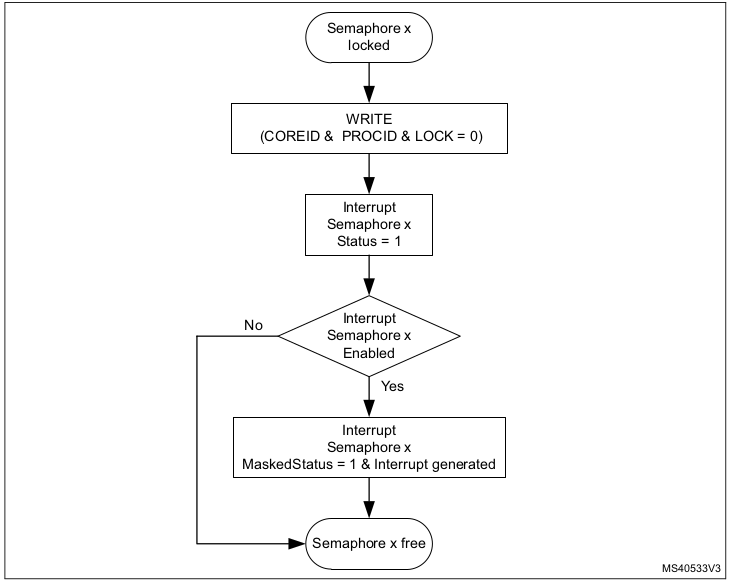
\includegraphics[width=150mm, keepaspectratio]{figures/hsem-interrupt.png}
    \caption{HSEM Interrupt State Diagram\cite{HsemInterrupt}}
    \label{fig:hsem-interrupt-sd}
\end{figure}

As an example, Listing~\ref{lst:interrupt-hsem-ex} shows the implementation of an interrupt handler that toggles an LED when any HSEM interrupt is triggered. There is only one source of interrupt for this peripheral, so one interrupt handler must serve the interrupts coming from all the semaphores. In the interrupt handler, we first query the list of masked freed semaphores then disable interrupt and finally clear the interrupt flags. After these steps, the interrupt handler can provide its normal functionality, which in this case is just toggling an LED.

\subsection{Limitations}

Dual-core functionality is not supported in underlying crates, only one of the two interrupt lines can be used. As one interrupt line is connected to each of the two cores, this means that through correct and safe code we are only able to handle HSEM interrupts on the M7 core.
